\section{JavaScript}

\begin{concept}{JavaScript Grundlagen}
    \begin{itemize}
        \item Veröffentlicht 1995 für Netscape Navigator 2.0
        \item Entwickelt von Brendan Eich
        \item Dynamisches Typenkonzept
        \item Objektorientierter und funktionaler Stil möglich
        \item Wichtigste Programmiersprache für Webanwendungen
        \item Läuft im Browser und serverseitig (Node.js)
    \end{itemize}
\end{concept}

\subsection{Grundlagen und Datentypen}

\begin{formula}{Web-Konsole}
    JavaScript Console im Browser und Node.js:
    \begin{itemize}
        \item \texttt{console.log(message)}: Gibt eine Nachricht aus
        \item \texttt{console.clear()}: Löscht die Konsole
        \item \texttt{console.trace(message)}: Stack trace ausgeben
        \item \texttt{console.error(message)}: stderr ausgeben
        \item \texttt{console.time()}: Timer starten
        \item \texttt{console.timeEnd()}: Timer stoppen
    \end{itemize}
\end{formula}

\begin{definition}{Datentypen}
    Primitive Datentypen:
    \begin{itemize}
        \item \texttt{number}: 64-Bit Floating Point (IEEE 754)
            \begin{itemize}
                \item \texttt{Infinity}: $1/0$
                \item \texttt{NaN}: Not a Number ($0/0$)
            \end{itemize}
        \item \texttt{bigint}: Ganzzahlen beliebiger Größe (mit n am Ende)
        \item \texttt{string}: Zeichenketten in \texttt{''}, \texttt{""} oder \texttt{``}
        \item \texttt{boolean}: \texttt{true} oder \texttt{false}
        \item \texttt{undefined}: Variable deklariert aber nicht initialisiert
        \item \texttt{null}: Variable bewusst ohne Wert
        \item \texttt{symbol}: Eindeutiger Identifier
    \end{itemize}
\end{definition}

\begin{KR}{typeof-Operator}
\begin{lstlisting}[language=JavaScript, style=basesmol]
typeof 42          // 'number'
typeof 42n         // 'bigint'
typeof "text"      // 'string'
typeof true        // 'boolean'
typeof undefined   // 'undefined'
typeof null        // 'object' (!)
typeof {}          // 'object'
typeof []          // 'object'
typeof (() => {})  // 'function'
typeof Infinity    // 'number'
typeof NaN         // 'number'
typeof 'number'    // 'string'
\end{lstlisting}
\end{KR}

\begin{theorem}{Variablenbindung}
    JavaScript kennt drei Arten der Variablendeklaration:
    \begin{itemize}
        \item \texttt{var}
            \begin{itemize}
                \item Scope: Funktions-Scope
                \item Kann neu deklariert werden
                \item Wird gehoistet
            \end{itemize}
        \item \texttt{let}
            \begin{itemize}
                \item Scope: Block-Scope
                \item Moderne Variante für veränderliche Werte
                \item Keine Neudeklaration im gleichen Scope
            \end{itemize}
        \item \texttt{const}
            \begin{itemize}
                \item Scope: Block-Scope
                \item Wert kann nicht neu zugewiesen werden
                \item Referenz ist konstant (Objekte können modifiziert werden)
            \end{itemize}
    \end{itemize}
\end{theorem}

\begin{formula}{Operatoren und Vergleiche}
    \begin{itemize}
        \item Arithmetische Operatoren: $+, -, *, /, \%, ++, --$
        \item Zuweisungsoperatoren: $=, +=, -=, *=, /=, \%=$
        \item Vergleichsoperatoren: 
            \begin{itemize}
                \item \texttt{==}, \texttt{!=}: Mit Typumwandlung
                \item \texttt{===}, \texttt{!==}: Ohne Typumwandlung (strikt)
            \end{itemize}
        \item Logische Operatoren: $\&\&, ||, !$
        \item Nullish Coalescing: \texttt{??}
        \item Optional Chaining: \texttt{?.}
    \end{itemize}
\end{formula}

\begin{KR}{Kontrollstrukturen}
\begin{lstlisting}[language=JavaScript, style=basesmol]
// If-Statement
if (condition) {
    // code
} else if (otherCondition) {
    // code
} else {
    // code
}

// Switch Statement
switch(value) {
    case 1:
        // code
        break;
    case 2:
        // code
        break;
    default:
        // code
}

// Loops
for (let i = 0; i < n; i++) { }
while (condition) { }
do { } while (condition);
for (let item of array) { }
for (let key in object) { }
\end{lstlisting}
\end{KR}

\subsection{Objekte und Arrays}

\begin{theorem}{Objekt vs Array}
    \begin{tabular}{|l|l|l|}
        \hline
        Was & Objekt & Array \\
        \hline
        Art & Attribut-Wert-Paare & Sequenz von Werten \\
        \hline
        Literalnotation & werte = \{a: 1, b: 2\} & liste = [1,2,3] \\
        \hline
        Ohne Inhalt & werte = \{\} & liste = [] \\
        \hline
        Elementzugriff & werte["a"] oder werte.a & liste[0] \\
        \hline
    \end{tabular}
\end{theorem}

\begin{KR}{Objekt-Manipulation}
\begin{lstlisting}[language=JavaScript, style=basesmol]
// Objekt erstellen
let person = {
    name: "John",
    age: 30,
    greet() {
        return `Hello, I'm ${this.name}`;
    }
};

// Eigenschaften manipulieren
person.job = "Developer";    // hinzufuegen
delete person.age;          // loeschen
"name" in person;           // true

// Objekte zusammenfuehren
Object.assign(person, {city: "Berlin"});

// Spread Syntax
let clone = {...person};

// Destrukturierung
let {name, job} = person;
\end{lstlisting}
\end{KR}

\begin{formula}{Array-Methoden}
    Wichtige Array-Operationen:
    \begin{itemize}
        \item \texttt{push()}, \texttt{pop()}: Ende hinzufügen/entfernen
        \item \texttt{unshift()}, \texttt{shift()}: Anfang hinzufügen/entfernen
        \item \texttt{splice()}: Elemente einfügen/entfernen
        \item \texttt{slice()}: Teilarray erstellen
        \item \texttt{map()}, \texttt{filter()}, \texttt{reduce()}: Funktional
        \item \texttt{forEach()}: Iteration über Elemente
        \item \texttt{join()}, \texttt{concat()}: Arrays verbinden
        \item \texttt{sort()}, \texttt{reverse()}: Sortieren/Umkehren
    \end{itemize}

    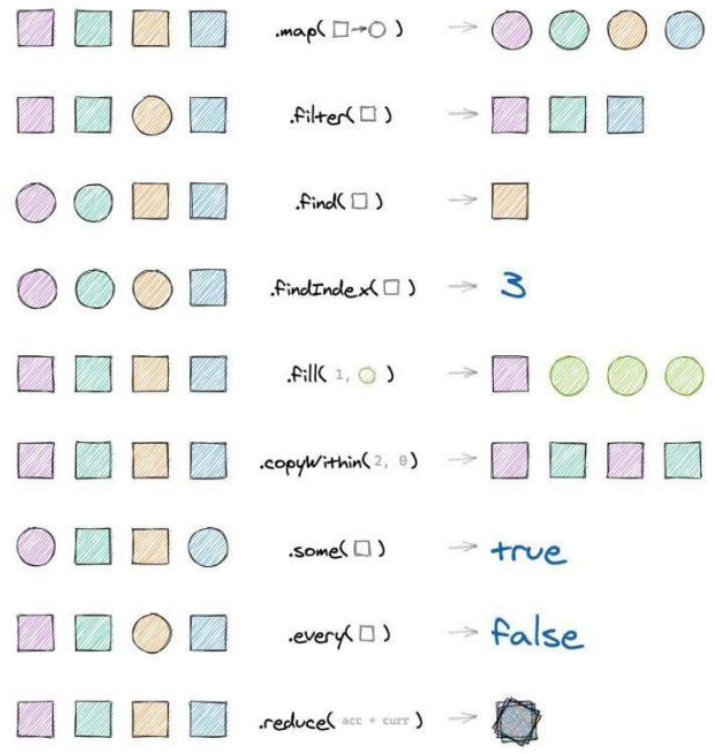
\includegraphics[width=0.5\linewidth]{images/array_cheatsheet.png}
\end{formula}

\begin{concept}{JSON}
    JavaScript Object Notation:
    \begin{itemize}
        \item Daten-Austauschformat, nicht nur für JavaScript
        \item Basiert auf JavaScript-Objektliteralen
        \item Methoden: \texttt{JSON.stringify()} und \texttt{JSON.parse()}
    \end{itemize}
\begin{lstlisting}[language=JavaScript, style=basesmol]
let obj = {type: "cat", name: "Mimi", age: 3};
let json = JSON.stringify(obj);
// '{"type":"cat","name":"Mimi","age":3}'

let parsed = JSON.parse(json);
// {type: 'cat', name: 'Mimi', age: 3}
\end{lstlisting}
\end{concept}

\subsection{Funktionen}

\begin{KR}{Funktionsdefinitionen}
\begin{lstlisting}[language=JavaScript, style=basesmol]
// Funktionsdeklaration
function add(a, b) {
    return a + b;
}

// Funktionsausdruck
const multiply = function(a, b) {
    return a * b;
};

// Arrow Function
const subtract = (a, b) => a - b;

// Arrow Function mit Block
const divide = (a, b) => {
    if (b === 0) throw new Error('Division by zero');
    return a / b;
};
\end{lstlisting}
\end{KR}

\begin{concept}{Parameter und Arguments}
    \begin{itemize}
        \item Default-Parameter: \texttt{function f(x = 1) \{\}}
        \item Rest-Parameter: \texttt{function f(...args) \{\}}
        \item Destrukturierung: \texttt{function f(\{x, y\}) \{\}}
        \item \texttt{arguments}: Array-ähnliches Objekt mit allen Argumenten
    \end{itemize}
\end{concept}

\begin{formula}{Funktionale Konzepte}
    \begin{itemize}
        \item Funktionen sind First-Class Citizens
        \item Können als Parameter übergeben werden
        \item Können von Funktionen zurückgegeben werden
        \item Closure: Zugriff auf umgebenden Scope
        \item Pure Functions: Keine Seiteneffekte
    \end{itemize}
\end{formula}

\begin{KR}{Closure Beispiel}
\begin{lstlisting}[language=JavaScript, style=basesmol]
function counter() {
    let count = 0;
    return {
        increment: () => ++count,
        decrement: () => --count,
        getCount: () => count
    };
}

const myCounter = counter();
myCounter.increment(); // 1
myCounter.increment(); // 2
myCounter.decrement(); // 1
\end{lstlisting}
\end{KR}

\begin{concept}{Prototypen}
    \begin{itemize}
        \item Jedes Objekt hat ein Prototyp-Objekt
        \item Prototyp dient als Fallback für Properties
        \item Vererbung über Prototypenkette
        \item \texttt{Object.create()} für Prototyp-Vererbung
    \end{itemize}
\end{concept}

\subsection{Asynchrone Programmierung}

\begin{concept}{Event Loop}
    \begin{itemize}
        \item JavaScript ist single-threaded
        \item Event Loop verarbeitet asynchrone Operationen
        \item Call Stack für synchronen Code
        \item Callback Queue für asynchrone Callbacks
        \item Microtask Queue für Promises und process.nextTick
    \end{itemize}
\end{concept}

\begin{KR}{Callbacks und Timer}
\begin{lstlisting}[language=JavaScript, style=basesmol]
// setTimeout
setTimeout(() => {
    console.log('Delayed by 1 second');
}, 1000);

// setInterval
const id = setInterval(() => {
    console.log('Every 2 seconds');
}, 2000);
clearInterval(id);

// Event Handler mit Callback
element.addEventListener('click', (event) => {
    console.log('Clicked!');
});
\end{lstlisting}
\end{KR}

\begin{KR}{Promises}
\begin{lstlisting}[language=JavaScript, style=basesmol]
// Promise erstellen
const myPromise = new Promise((resolve, reject) => {
    // Asynchrone Operation
    if (success) {
        resolve(result);
    } else {
        reject(error);
    }
});

// Promise verwenden
myPromise
    .then(result => {
        // Erfolgsfall
    })
    .catch(error => {
        // Fehlerfall
    })
    .finally(() => {
        // Wird immer ausgefuehrt
    });

// Promise.all
Promise.all([promise1, promise2])
    .then(results => {
        // Array mit allen Ergebnissen
    });

// Promise.race
Promise.race([promise1, promise2])
    .then(firstResult => {
        // Erstes erfuelltes Promise
    });
\end{lstlisting}
\end{KR}

\begin{KR}{Async/Await}
\begin{lstlisting}[language=JavaScript, style=basesmol]
// Async Funktion
async function getData() {
    try {
        const response = await fetch(url);
        const data = await response.json();
        return data;
    } catch (error) {
        console.error('Error:', error);
    }
}

// Parallele Ausfuehrung
async function getMultipleData() {
    const [data1, data2] = await Promise.all([
        getData(url1),
        getData(url2)
    ]);
    return { data1, data2 };
}
\end{lstlisting}
\end{KR}

\subsection{Node.js und Module}

\begin{concept}{Node.js}
    \begin{itemize}
        \item JavaScript Runtime basierend auf V8
        \item Event-driven und non-blocking I/O
        \item Großes Ökosystem (npm)
        \item Ideal für Netzwerk-Anwendungen
        \item REPL für interaktive Entwicklung
    \end{itemize}
\end{concept}

\begin{KR}{Module System}
\begin{lstlisting}[language=JavaScript, style=basesmol]
// CommonJS (Node.js)
const fs = require('fs');
module.exports = { /* ... */ };

// ES Modules
import { function1 } from './module.js';
export const variable = 42;
export default class MyClass { /* ... */ }

// package.json
{
    "type": "module",
    "dependencies": {
        "express": "^4.17.1"
    }
}
\end{lstlisting}
\end{KR}

\begin{formula}{NPM Commands}
    Wichtige npm Befehle:
    \begin{itemize}
        \item \texttt{npm init}: Projekt initialisieren
        \item \texttt{npm install}: Abhängigkeiten installieren
        \item \texttt{npm install --save package}: Produktiv-Dependency
        \item \texttt{npm install --save-dev package}: Entwicklungs-Dependency
        \item \texttt{npm run script}: Script ausführen
        \item \texttt{npm update}: Packages aktualisieren
    \end{itemize}
\end{formula}

\subsection{Testing mit Jasmine}

\begin{concept}{Test-Driven Development}
    \begin{itemize}
        \item Tests vor Implementation schreiben
        \item Red-Green-Refactor Zyklus
        \item Tests als Spezifikation
        \item Bessere Code-Qualität
        \item Einfacheres Refactoring
    \end{itemize}
\end{concept}

\begin{KR}{Jasmine Tests}
\begin{lstlisting}[language=JavaScript, style=basesmol]
describe("Calculator", () => {
    let calc;
    
    beforeEach(() => {
        calc = new Calculator();
    });
    
    it("should add numbers", () => {
        expect(calc.add(1, 2)).toBe(3);
    });
    
    it("should throw on division by zero", () => {
        expect(() => {
            calc.divide(1, 0);
        }).toThrow();
    });
});
\end{lstlisting}
\end{KR}

\begin{formula}{Jasmine Matchers}
    \begin{itemize}
        \item \texttt{toBe()}: Strikte Gleichheit (===)
        \item \texttt{toEqual()}: Strukturelle Gleichheit
        \item \texttt{toContain()}: Array/String enthält Element
        \item \texttt{toBeDefined()}, \texttt{toBeUndefined()}
        \item \texttt{toBeTruthy()}, \texttt{toBeFalsy()}
        \item \texttt{toBeGreaterThan()}, \texttt{toBeLessThan()}
        \item \texttt{toMatch()}: RegExp Match
        \item \texttt{toThrow()}: Exception wird geworfen
    \end{itemize}
\end{formula}

\begin{KR}{Jasmine Setup}
\begin{lstlisting}[language=JavaScript, style=basesmol]
// Installation
npm install --save-dev jasmine

// jasmine.json
{
    "spec_dir": "spec",
    "spec_files": [
        "**/*[sS]pec.js"
    ],
    "helpers": [
        "helpers/**/*.js"
    ]
}

// Test ausführen
npx jasmine
\end{lstlisting}
\end{KR}